\documentclass{beamer}


\usepackage{amsmath}
\usepackage[style=alphabetic,url=true]{biblatex}
\usepackage{environ}
\usepackage{geometry}
\usepackage{graphicx}
\usepackage{tikz}
\usepackage[T2A]{fontenc}
\usepackage[utf8]{inputenc}
\usepackage[cache=false]{minted}
\usepackage{amsmath}
\usepackage{amsfonts}
\usepackage{amssymb}
\usepackage{calrsfs}
\usepackage{animate}
\usepackage{xmpmulti}


% \usetheme{Bergen}

\usecolortheme{beaver}

\setbeamertemplate{itemize item}[circle]
\setbeamertemplate{itemize subitem}{--}
\addtobeamertemplate{navigation symbols}{}{
  \usebeamerfont{footline}%
  \usebeamercolor[fg]{footline}%
  \hspace{1em}%
  \insertframenumber/\inserttotalframenumber
}
\graphicspath{ {./graphics/} }
\setminted[Python]{
  fontsize=\tiny
}
\setminted[Lisp]{
  fontsize=\tiny
}
\BeforeBeginEnvironment{minted}{\medskip}
\AfterEndEnvironment{minted}{\medskip}
\usetikzlibrary{matrix}
\tikzset{
  stack/.style={
    matrix of nodes,
    nodes={
      fill=lightgray,draw,text=black,font=\sffamily\bfseries,
      text height=11pt,text depth=3pt,baseline=center, minimum width=1cm
    },
    column sep=-\pgflinewidth/2
  }
}

\title{
  Біткоїн та криптовалютні технології \\
  Лекція 10: Масштабування Біткоїна 2/2
}

\author{Юрій Жикін}
\date{5 травня, 2025}

\begin{document}

\frame{\titlepage}

\begin{frame}
  \frametitle{Протоколи другого рівня}
  \begin{itemize}
  \item Контракти (Транзакції) виконуються в межах протоколу-надбудови, а
    основна Біткоїн-мережа (ланцюг блоків) використовується як рівень
    фіналізації контрактів.
  \item Підписана Біткоїн-транзакція — це платіж, який можна ``заявити'' шляхом
    публікації її в мережі Bitcoin.
  \item Платежі другого рівня можуть бути реалізовані за допомогою підписаних
    транзакцій, які публікуються лише у разі необхідності фіналізації.
  \item До моменту публікації \textbf{фіналізуюючої транзакції},
    \textbf{повторне витрачання коштів} все ще можливе.
  \end{itemize}
\end{frame}

\begin{frame}
  \frametitle{Платіжні канали 1/2}
  \begin{itemize}
  \item \textbf{Платіжний канал} — це конструкція, яка дозволяє \textbf{двом}
    сторонам здійснювати платежі без надсилання транзакцій до Біткоїн-мережі.
  \item \textbf{Двосторонній платіжний канал} дещо подібний до платіжного
    чека, який розподіляє спільний банківський рахунок між двома сторонами.
    \begin{itemize}
    \item спільний банківський рахунок з балансом $N$ одиниць;
    \item обидві сторони A і B ``володіють'' частинами балансу по $N/2$;
    \item обидві сторони підписують чек, що виплачує по $N/2$ одиниць A і B;
    \item коли сторона A хоче заплатити $M$ одиниць стороні B, вони
      \textbf{підписують новий чек}, який виплачує $N/2 - M$ стороні A та
      $N/2 + M$ стороні B, та \textbf{знищують старі чеки}.
    \end{itemize}
  \end{itemize}
\end{frame}

\begin{frame}
  \frametitle{Платіжні канали 2/2}
  \begin{itemize}
  \item Існує кілька пропозицій: канали Спіллмана, CLTV, канали Пуна-Драйї,
    дуплексні платіжні канали Деккера-Ваттенхофера, канали eltoo Деккера-Рассела-Осунтокуна.
  \item Платіжні канали Пуна-Драйї були представлені в оригінальній публікації.
  \item Кошти, що лежать в основі каналу, блокуються мультипідписом 2-з-2.
  \item Ще до того, як фінансуюча транзакція підписується, спочатку створюються
    й підписуються транзакції-зобов’язання (commitment) для кожної сторони.
  \item Оскільки потрібно посилатися на транзакції, які ще не підписані,
    необхідно формат транзакцій, що відокремлюють підписи від частини
    транзакції, яка хешується для створення txid (Segregated Witness).
  \end{itemize}
\end{frame}

\begin{frame}[fragile]
  \frametitle{Мережа Lightning 1/4}
  \begin{itemize}
  \item Мережа двосторонніх платіжних каналів, яка дозволяє здійснювати
    багатоетапні платежі, передаючи кошти через послідовність платіжних каналів.
  \item Запропонована у 2015 році; почала працювати на початку 2018 року.
  \end{itemize}
  \begin{center}
    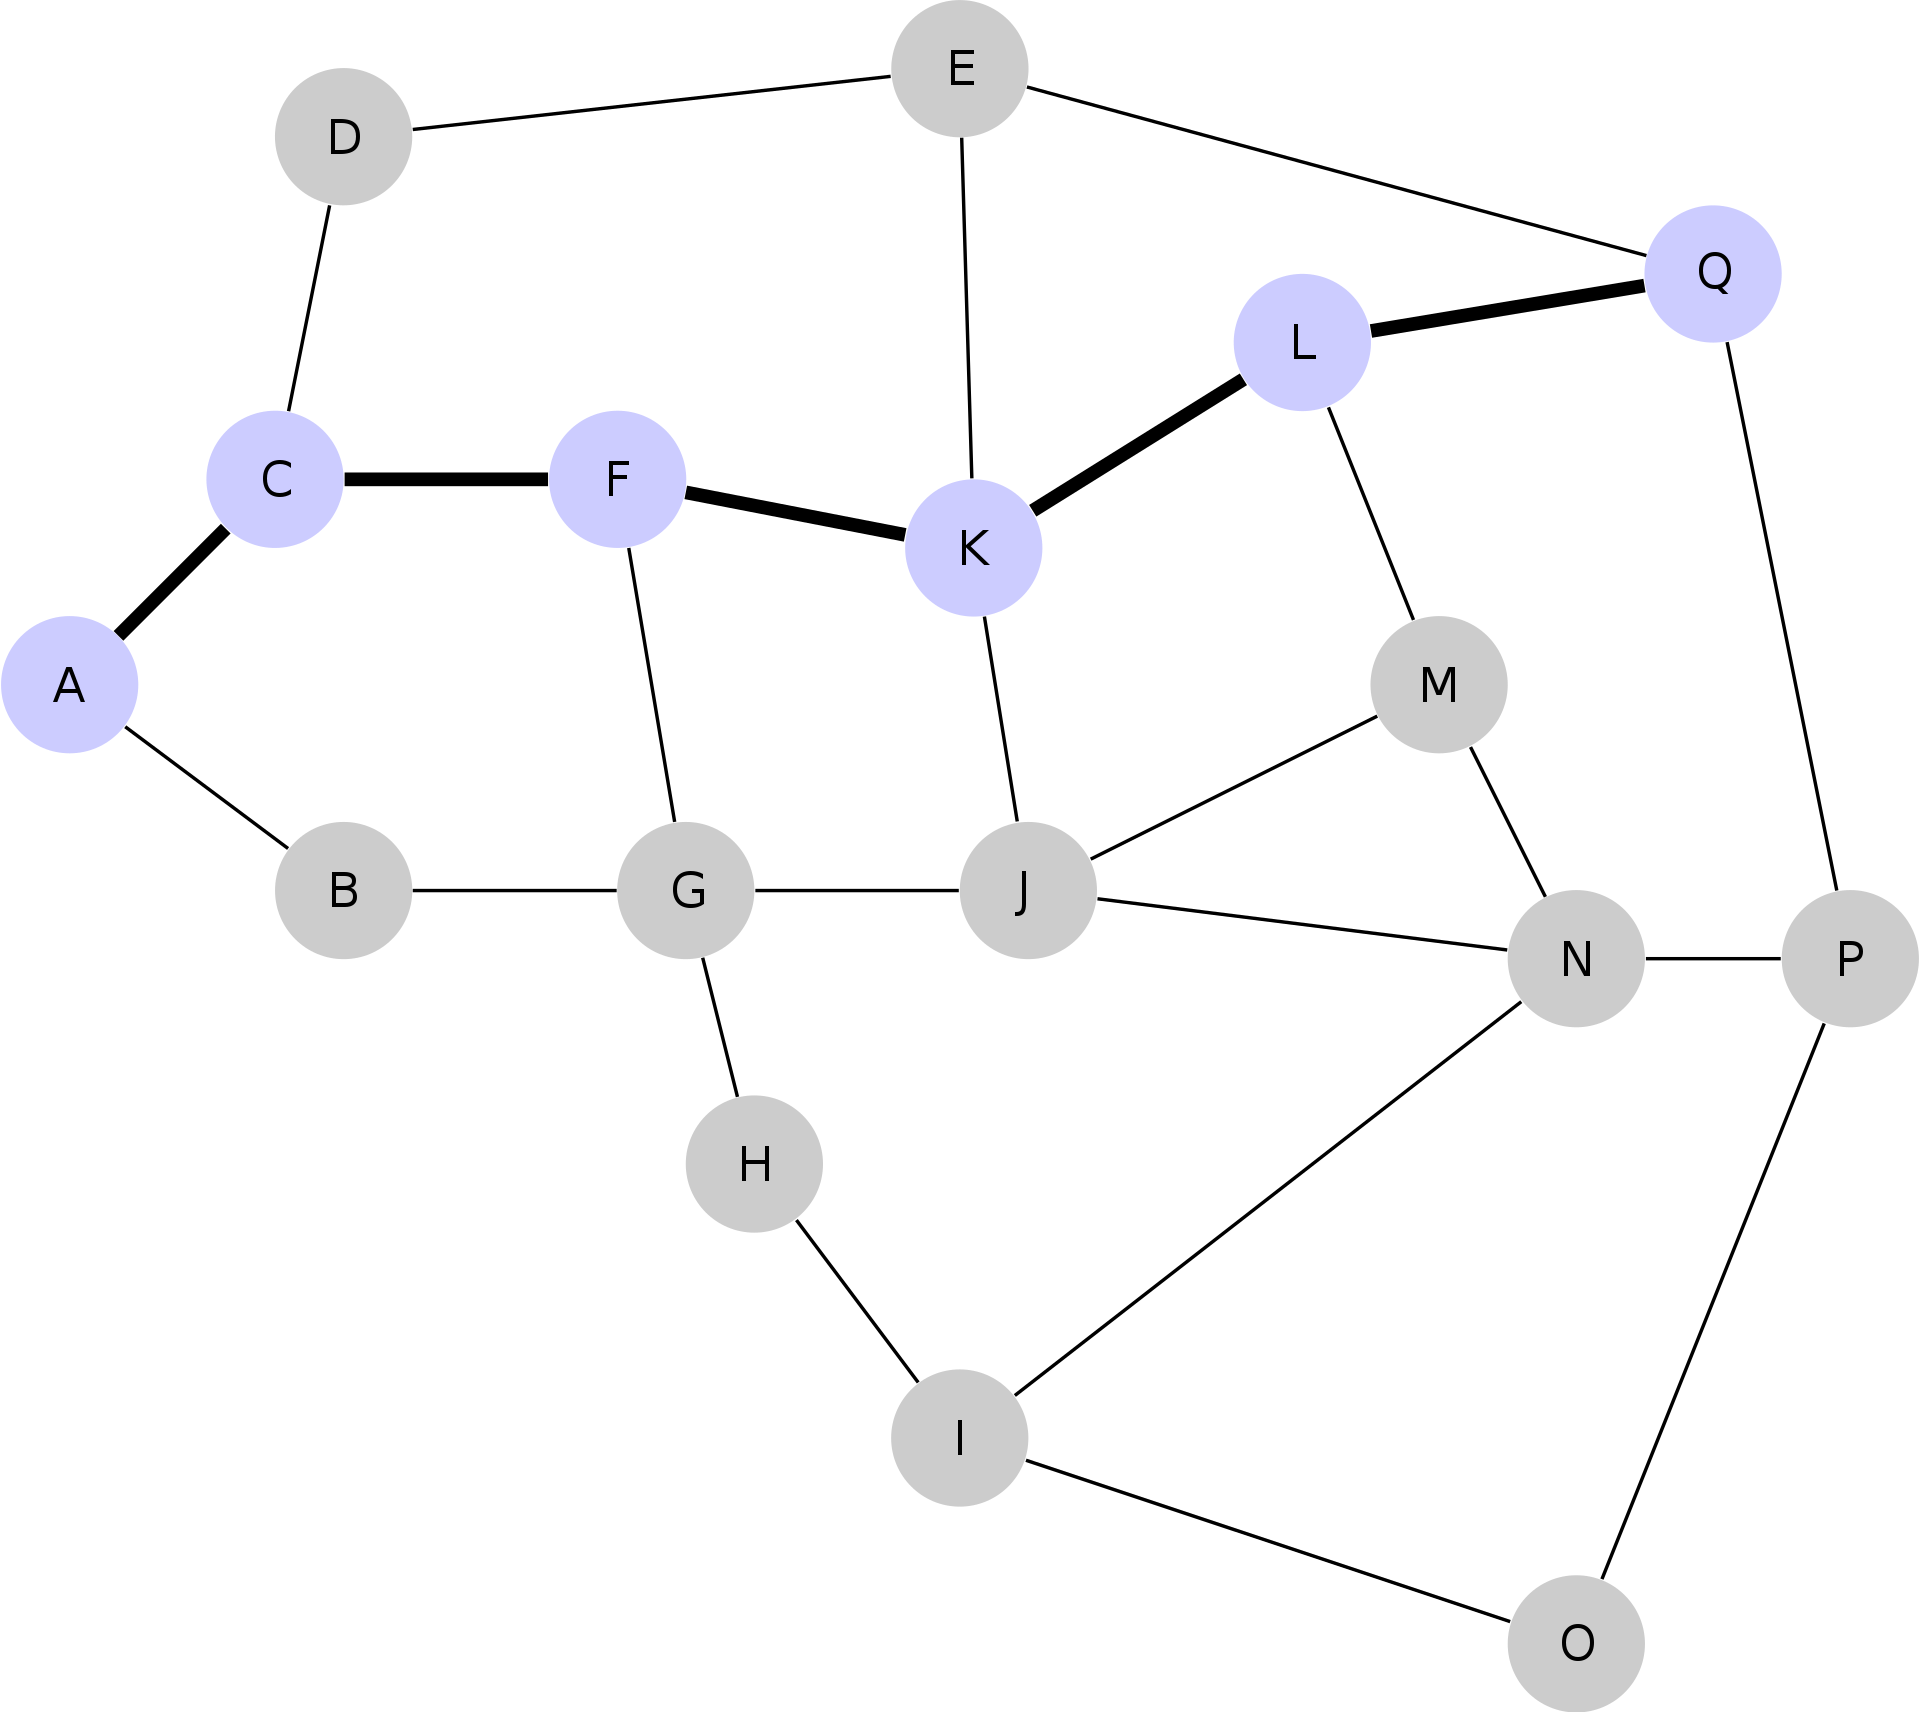
\includegraphics[width=0.5\textwidth]{ln}
  \end{center}
\end{frame}

\begin{frame}[fragile]
  \frametitle{Мережа Lightning 2/4}
  \begin{itemize}
  \item Кожен канал — це ``спільний рахунок'' з мультипідписом 2-з-2
  \item Фінансуюча транзакція:
    \begin{minted}{Lisp}
      OP_2 <A public key> <B public key> OP_2 OP_CHECKMULTISIG
    \end{minted}
  \end{itemize}
\end{frame}

\begin{frame}[fragile]
  \frametitle{Мережа Lightning 3/4}
  \begin{itemize}
  \item Одразу створюються дві транзакції-зобов'язання — по одній для кожного
    учасника.
  \item Вихід для віддаленої сторони виглядає так:
    \begin{minted}{Lisp}
      <remote public key> OP_CHECKSIG
    \end{minted}
  \item Вихід для локальної сторони виглядає так:
    \begin{minted}{Lisp}
      OP_IF
          <revocation public key>
      OP_ELSE
          <delay> OP_CHECKSEQUENCEVERIFY OP_DROP
          <local delayed pubkey>
      OP_ENDIF
      OP_CHECKSIG          
    \end{minted}
  \end{itemize}
\end{frame}

\begin{frame}[fragile]
  \frametitle{Мережа Lightning 2/2}
  \begin{itemize}
  \item Сутність $A$ хоче заплатити сутності $B$, і в мережі існує шлях між ними: 
    $A, C_1, C_2, ..., C_n, B$:
    \begin{itemize}
    \item $B$ генерує випадкове значення $R$, обчислює хеш $H = hash(R)$ і 
      передає $H$ сутності $A$;
    \item $A$ створює додатковий HTLC (контракт з хеш-таймлоком) і оновлює 
      свій канал із $C_1$:
      \begin{minted}{Lisp}
        OP_IF
          HASH160 <H> OP_EQUAL
          <B public key> OP_CHECKSIG
        OP_ELSE
          <locktime> OP_CHECKLOCKTIMEVERIFY
          <A public key> OP_CHECKSIG
        OP_ENDIF
      \end{minted}
    \item $C_1$ оновлює свій платіжний канал із $C_2$ і так далі, доки $C_n$ не 
      оновить канал із $B$.
    \item $B$ передає $R$ до $C_n$ і отримує кошти; $C_n$ передає $R$ до
      $C_{n-1}$ і так далі, доки $C_1$ не отримає кошти від $A$.
    \end{itemize}
  \end{itemize}
\end{frame}

\begin{frame}
  \frametitle{Використання мережі Lightning}
  \begin{itemize}
  \item 11,380 вузлів (20,478 вузлів у 2021 році),
  \item 42,459 каналів (45,774 канали у 2021 році),
  \item 4,230.60 BTC = \$400,334,511 (1,332.25 BTC = \$52,290,595 у 2021 році),
  \item Тривають дослідження, удосконалення та розробка нових функцій,
  \item Ігри, онлайн-магазини та інші бізнеси.
  \end{itemize}
\end{frame}

\begin{frame}
  \frametitle{Рекомендовані ресурси}
  \begin{itemize}
  \item \textbf{Basis of Lightning Technology}
    \begin{itemize}
    \item  https://github.com/lightning/bolts
    \end{itemize}
  \item \textbf{Mastering the Lightning Network}
    \begin{itemize}
    \item by Andreas Antonopoulos, Olaoluwa Osuntokun, and René Pickhardt.
    \item https://github.com/lnbook/lnbook
    \end{itemize}
  \end{itemize}
\end{frame}

\begin{frame}
  \frametitle{Кінець}
  \begin{center}
    Дякую за увагу!
  \end{center}
\end{frame}

\end{document}

%%% Local Variables:
%%% mode: latex
%%% TeX-master: t
%%% End:
